\begin{figure}
\begin{center}

\begin{subfigure}[b]{\columnwidth}
\centering
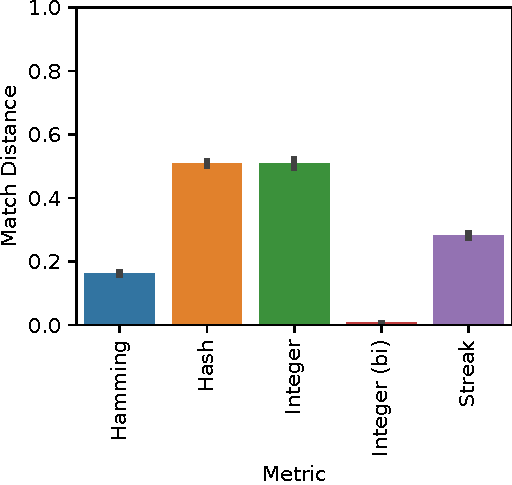
\includegraphics[width=\columnwidth]{{{sphere/bitweight=0.5+seed=1+title=dimensionality_barplot+_data_hathash_hash=c0f6c5cf854ff253+_script_fullcat_hash=03ce1e318a24a109+ext=}}}
\caption{
Mean statistic values for each metric.
Error bars represent 95\% confidence intervals.
}
\label{fig:sphere_distnplot}
\end{subfigure}

\vspace{2ex}

\begin{subfigure}[b]{\columnwidth}
\centering
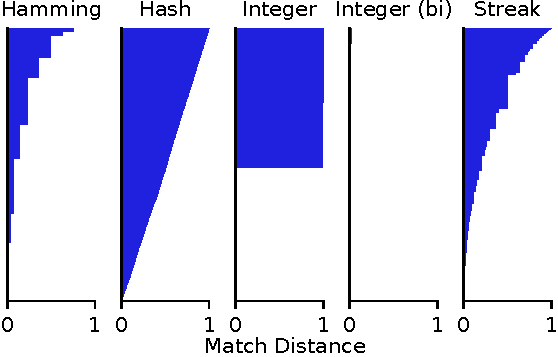
\includegraphics[width=\columnwidth]{{{sphere/bitweight=0.5+seed=1+title=dimensionality_distnplot+_data_hathash_hash=c0f6c5cf854ff253+_script_fullcat_hash=03ce1e318a24a109+ext=}}}
\caption{
Statistic distribution, where each horizontal bar sliver represents one independent observation.
}
\label{fig:sphere_barplot}
\end{subfigure}

\caption{
Dimensionality statistic measured as distances between two tags sampled from within 0.01 match distance of a third tag.
}
\label{fig:sphere}

\end{center}
\end{figure}
